\documentclass[tikz]{standalone}

\usepackage{amsfonts}
\usepackage{amsmath}
\usepackage{braket}

\usepackage{tikz}
\usetikzlibrary{arrows, arrows.meta, calc, decorations, positioning}

% load TikZ grafic definitions
%\input{gfx_TikZ}

% main document
\begin{document}

	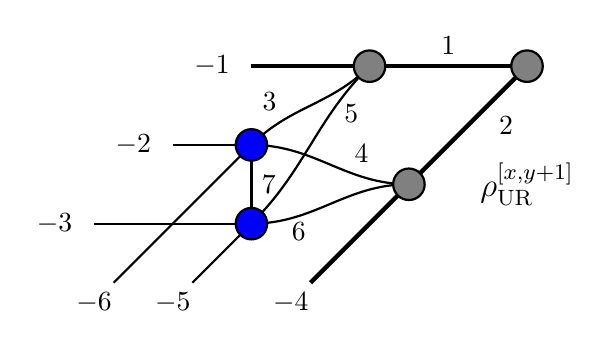
\begin{tikzpicture}[]

	\def\tensorSize{0.2}

		\begin{scope}[shift = {(+3, +2)}]

			% label
			\node at (+3.5,0) {\large$\rho_\text{UR}^{[x,y + 1]}$};

			% network corrdinates
			\coordinate (PN) at (+0.0, +0.5);
			\coordinate (PC) at (+0.0, -0.5);
			\coordinate (T1) at (+1.5, +1.5);
			\coordinate (C2) at (+3.5, +1.5);
			\coordinate (T2) at (+2.0, -0.0);
			
			% external links
			\draw[ultra thick] (T1) to ($(T1) + (-1.50, +0.00)$) node at ($(T1) + (-2.00, +0.00)$) {$-1$};
			\draw[thick] (PN) to ($(PN) + (-1.00, +0.00)$) node at ($(PN) + (-1.50, +0.00)$) {$-2$};
			\draw[thick] (PC) to ($(PC) + (-2.00, +0.00)$) node at ($(PC) + (-2.50, +0.00)$) {$-3$};
			\draw[ultra thick] (T2) to ($(T2) + (-1.25, -1.25)$) node at ($(T2) + (-1.50, -1.50)$) {$-4$};
			\draw[thick] (PC) to ($(PC) + (-0.75, -0.75)$) node at ($(PC) + (-1.00, -1.00)$) {$-5$};
			\draw[thick] (PN) to ($(PN) + (-1.75, -1.75)$) node at ($(PN) + (-2.00, -2.00)$) {$-6$};
			

			% internal links
			\draw[ultra thick] (C2) to (T2) node[right = 0.25] at ($(C2)!0.5!(T2)$) {$2$};
			\draw[thick] (T2) to [out = 180, in =   0] (PC) node[below] at ($(T2)!0.7!(PC)$) {$6$};
			\draw[ultra thick] (C2) -- (T1) node [midway, above] {$1$};
			\draw[thick] (T1) to [out = 225, in = 45] (PC) node[right] at ($(T1)!0.3!(PC)$) {$5$};
			\draw[thick] (T2) to [out = 180, in =   0] (PN) node[above] at ($(T2)!0.3!(PN)$) {$4$};
			\draw[thick] (T1) to [out = 225, in = 45] (PN) node[above left] at ($(T1)!0.7!(PN)$) {$3$};
			\draw[thick] (PN) -- (PC) node [midway, right] {$7$};

			% CTMRG tensors
			\foreach \tensor in {T1, C2, T2} {
				\draw[thick,black,fill = gray] (\tensor) circle (\tensorSize);
			}

			% iPEPS tensors
			\foreach \tensor in {PN, PC} {
				\draw[thick,black,fill = blue] (\tensor) circle (\tensorSize);
			}
			
		\end{scope}

	\end{tikzpicture}

\end{document}

%%% Local Variables:
%%% mode: latex
%%% TeX-master: t
%%% End:
